% =====================================================================
% IPCO 2027 extended abstract -- Learning-Augmented Benders Decomposition
% Format: Springer LNCS (llncs.cls v2.24), double-blind.
% Main body (Sections 1-6): at most 12 pages in LNCS format.
% After the main body: acknowledgements, references, appendix (no limit).
% See README.md for the full IPCO 2027 rules and checklist.
% =====================================================================
\documentclass[runningheads]{llncs}

% ---- Packages (keep LNCS look: do not change fonts, margins or spacing) ----
\usepackage[T1]{fontenc}
\usepackage{amsmath,amssymb}
\usepackage{graphicx}
\usepackage{pgfplots}
\usepgfplotslibrary{groupplots}
\pgfplotsset{compat=1.18}
\usepackage{booktabs}
\usepackage{multirow}
\usepackage{array}
\usepackage{algorithm}
\usepackage[noend]{algpseudocode}
\usepackage{xcolor}
\usepackage[hidelinks]{hyperref}
\usepackage[capitalise,noabbrev]{cleveref}

% llncs.cls already defines theorem, lemma, proposition, corollary,
% definition, remark, example and proof. Add only what is missing.
\spnewtheorem{assumption}{Assumption}{\bfseries}{\itshape}

% ---- Drafting helpers (remove before submission) ----
\newcommand{\todo}[1]{\textcolor{red}{[TODO: #1]}}
% Review markup: reviewer comments in blue (\textcolor{blue}{...}), text revised
% in response in purple. \rev{...} for short inline text; revblock for passages
% that span paragraphs, equations or environments.
\newcommand{\rev}[1]{\textcolor{purple}{#1}}
\newcommand{\fillin}{\textcolor{red}{\underline{\hspace{2em}}}}% number to be filled after the runs
\newenvironment{revblock}{\color{purple}}{}

% ---- Notation (fill in from the journal manuscript as we port content) ----
\newcommand{\R}{\mathbb{R}}
\newcommand{\E}{\mathbb{E}}


\begin{document}

\title{Learning-Augmented Benders Decomposition\\ with Performance Guarantees}
\titlerunning{Learning-Augmented Benders Decomposition}

% ---- Double-blind: keep anonymous for submission ----------------------
\author{Anonymous Author(s)}
\authorrunning{Anonymous}
\institute{Anonymous Institution(s)}
% For the camera-ready version only (after acceptance), replace with:
% \author{First Author\inst{1} \and Second Author\inst{1} \and Third Author\inst{2}}
% \institute{...}

\maketitle

\begin{abstract}
% Abstract (LNCS: 150--250 words). Title and abstract go on the first page.
The Benders decomposition (BD) method can become computationally expensive for large two-stage stochastic programs because each iteration may require solving a large number of subproblems. We propose Learning-Augmented Benders Decomposition (LABD), which solves only a selected subset of subproblems exactly and predicts dual-feasible solutions for the remaining ones. After a short warm-up phase, LABD learns representations of subproblem behavior, uses them to select the exact subproblems, and trains a mapping that predicts the dual solution of each remaining subproblem from its representation and its current state. Infeasible predictions are certified without solving an optimization problem: an explicit step along the segment from the mean of the current exact duals moves toward the prediction as far as dual feasibility allows, and only if it improves the dual objective. Because only dual-feasible predictions are used for cut generation, the resulting optimality cuts remain valid. We establish optimality-gap bounds that separate the contribution of the exact subproblems from that of the learned prediction. On stochastic capacitated facility location instances with 100 to 500 scenarios, LABD matches the objective value of Standard BD in 34 of the 36 configurations that Standard BD solves while reducing the median solution time by about 78\% (a speedup of about $4.6\times$), whereas solving a random subset exactly and averaging its duals is not faster than Standard BD in the median.

\keywords{Benders decomposition \and Two-stage stochastic programming \and Machine learning \and Dual prediction}
\end{abstract}

% ---------------------------- MAIN BODY (<= 12 pages) ----------------------------
\section{Introduction}\label{sec:intro}

Benders decomposition is a standard tool for large two-stage programs: the first-stage decisions stay in a master problem, the second stage splits into independent blocks or scenarios, and dual extreme points of the blocks generate optimality cuts that refine the master~\cite{geoffrion1970elements,birge2006introduction,rahmaniani2017benders}. In the multi-cut version, every subproblem is solved at every iteration. With hundreds of scenarios, these solves dominate the running time.

Exact solves are not needed for validity. Any dual-\emph{feasible} vector of a subproblem gives a valid, possibly weaker, cut~\cite{zakeri2000inexact,yang2012tighter}. This creates a trade-off between how strong the dual information behind a cut is and how much it costs to obtain, and it suggests a role for learning: solve a few subproblems exactly, and infer dual-feasible vectors for the others from what has been observed. Three things must hold for this to work. The predictor must use information that is actually available when a cut is needed; its output must be certified dual feasible, otherwise the cut is invalid; and the certification must be cheap, otherwise nothing is saved.

We propose \emph{Learning-Augmented Benders Decomposition} (LABD). After a short warm-up in which all subproblems are solved exactly, LABD learns a representation of each subproblem from the trajectory of its optimal duals, fixes a small set of subproblems to be solved exactly, and trains a mapping that predicts the dual vector of every other subproblem from its representation and from its current dual objective. A raw prediction may be infeasible. Restoring feasibility by optimization means either solving the subproblem itself or solving a linear program that finds a nearby dual-feasible vector; both are posed over the same dual polyhedron, so either one costs about as much as the exact solve that prediction was meant to avoid. We show that a single dual-feasible reference point removes this cost: moving from the reference point toward the prediction for as long as the dual constraints allow gives a feasible vector, and the length of this move is given by an explicit formula. The same move can be chosen so that the resulting cut is never weaker than the cut of the reference point at the current first-stage solution. We exploit the structure of the problem, a dual feasible region shared by all subproblems, to obtain such a reference point at every iteration from the subproblems that are solved exactly.

\subsection{Related Work}\label{subsec:related}

Inexact Benders methods use dual-feasible, non-optimal solutions and keep convergence under suitable conditions~\cite{zakeri2000inexact}; such cuts need not come from extreme points and may be weaker~\cite{yang2012tighter}. Sampling reduces the second-stage information evaluated per iteration~\cite{infanger1992monte}, and Bertsimas et al.~\cite{bertsimas2024stochastic} solve a random sample of scenarios and construct deterministic valid cuts for the rest by aggregating the sampled duals. LABD shares the premise that useful cuts do not require an optimal dual for every subproblem at every iteration. It differs in that the dual vector of each unsolved subproblem is predicted from subproblem-specific information and the current state, and is then certified.

Learning has been used inside Benders decomposition to propose master solutions that are then evaluated by the usual Benders steps~\cite{mana2024accelerating,agyeman2026graph}, and to decide which already-generated cuts to keep, by classification~\cite{jia2021benders} or reinforcement learning~\cite{cai2026rlbd}; related work in general cutting-plane methods learns which separators to run, when to stop, or which cuts to add~\cite{li2023separators,ling2024stop,huang2022learning,paulus2022learning}. In all of these, the subproblem information behind a cut must still be computed. Closer to LABD is work that learns the cut-generation oracle itself. Neural Benders learns which optimal dual to use for a degenerate subproblem that is being solved~\cite{monemi2025neuralbenders}. Learned value functions and multipliers yield approximate generalized Benders cuts~\cite{mitrai2024mlbenders}; KKT-informed networks predict primal--dual subproblem solutions and use them as inexact cuts~\cite{agyeman2026hybrid}; and learned duals with a safe shift have been used in nested Benders~\cite{aslani2025lcc}. Learned recourse functions have also been embedded directly in two-stage models~\cite{patel2022neur2sp}.  Larsen et al.~\cite{larsen2024fast} replace exact second-stage solutions in the L-shaped method by supervised predictions trained in advance on similar instances, which yields fast heuristics with a small loss in accuracy; LABD instead learns within the instance being solved, from its own warm-up, keeps a subset of subproblems exact, and certifies every predicted dual so that all cuts remain valid.

When learned information defines a cut, validity becomes the central issue. Proxy-BD~\cite{guan2026proxy} learns a stand-alone proxy of the subproblem response and passes its output through a predict--project--complete layer that returns dual-feasible certificates. LABD also separates validity from prediction accuracy, but its certificate needs no projection: feasibility is restored by a single explicit step toward the prediction from a reference point built from the exact duals of the current iteration, a step that exploits the relationships among subproblems of the same instance. The certificate also comes with a bound on the resulting loss in solution quality.

\subsection{Our Contributions}\label{subsec:contributions}
\begin{itemize}
\item We extract the learning information from the Benders process itself: during warm-up, exact dual responses are collected across subproblems and first-stage solutions, and their trajectories yield subproblem representations through graph embeddings, with little reliance on externally supplied features.
\item We develop LABD, which solves a representative subset of subproblems exactly and generates dual-feasible predictions for the others within one Benders procedure, so that every generated cut remains valid.
\item We give a certification step that turns any prediction into a dual-feasible vector without solving an optimization problem, using a reference point formed from the current exact duals, and chooses the step so that the predicted cut is never weaker than the cut of the reference point where it is generated.
\item We establish optimality-gap bounds that separate a structural term, which depends only on how far the predicted subproblems are from the exact ones, from a nonnegative term contributed by learning, together with a gap certificate that can be computed at the returned solution.
\item We evaluate LABD on stochastic capacitated facility location instances with 100 to 500 scenarios. Compared with Standard BD, LABD reduces the median solution time by about 78\% (a speedup of about $4.6\times$) and returns the optimal objective in 34 of the 36 configurations that Standard BD solves, and it is faster than the random-selection benchmark that solves the same number of subproblems exactly in 33 of them.
\end{itemize}


\section{Classical and Learning-Augmented Benders Decomposition}\label{sec:setting}

We consider the following class of two-stage mixed-integer linear programs with a block-separable linear second stage:
\begin{equation}\label{eq:two-stage}
\min_{\mathbf x\in\mathcal X}\;V(\mathbf x):=\mathbf c^\top\mathbf x+\sum_{m\in\mathcal M}\omega_m Q_m(\mathbf x),
\end{equation}
where
\begin{align}
Q_m(\mathbf x):=\min_{\mathbf y^m\ge\mathbf 0}\quad & \mathbf q^\top\mathbf y^m \label{eq:recourse}\\
\text{s.t.}\quad & \mathbf W\mathbf y^m\le\mathbf h_m-\mathbf T_m\mathbf x. \nonumber
\end{align}

Here, $\mathbf x\in\mathcal X\subseteq\R^{n_x}\times\mathbb Z^{n_z}$ contains the first-stage decisions, while $\mathbf y^m$ contains the second-stage decisions associated with block $m\in\mathcal M$. The vectors $\mathbf h_m$ and matrices $\mathbf T_m$ contain block-specific data, whereas $\mathbf W$ and $\mathbf q$ define the common second-stage structure. The coefficient $\omega_m>0$ denotes the weight associated with block $m$. In the stochastic case, $\mathcal M$ indexes a finite set of scenarios and $\omega_m$ is the probability of scenario $m$. Throughout, we assume $\mathbf q\ge\mathbf 0$ and relatively complete recourse, so that $0\le Q_m(\mathbf x)<\infty$ for all $\mathbf x\in\mathcal X$ and $m\in\mathcal M$.

\subsection{Classical Multi-cut Benders Decomposition}\label{subsec:classical-bd}

For a fixed first-stage solution $\mathbf x$, the second-stage problems are independent across $m\in\mathcal M$, and their dual representation is
\begin{equation}\label{eq:dual-subproblem}
Q_m(\mathbf x)=\max_{\boldsymbol\lambda\in\mathcal D}\ \boldsymbol\lambda^\top\mathbf g_m(\mathbf x),
\end{equation}
where
\begin{equation}\label{eq:dual-set-state}
\mathcal D:=\bigl\{\boldsymbol\lambda\in\R_+^r:\ \mathbf W^\top\boldsymbol\lambda\ge-\mathbf q\bigr\},
\qquad
\mathbf g_m(\mathbf x):=\mathbf T_m\mathbf x-\mathbf h_m .
\end{equation}

Since $\mathbf W$ and $\mathbf q$ do not depend on $m$, the feasible set $\mathcal D$ is identical across subproblems; only the dual objective $\mathbf g_m(\mathbf x)$, which we call the \emph{dual-objective state}, varies with $m$ and $\mathbf x$, and it is available as soon as $\mathbf x$ is known. Let $\Lambda:=\operatorname{ext}(\mathcal D)$. Any $\boldsymbol\lambda\in\mathcal D$ defines a valid lower supporting function of $Q_m$, and the extreme points in $\Lambda$ suffice to represent $Q_m$ exactly. Multi-cut Benders decomposition~\cite{geoffrion1970elements,rahmaniani2017benders} therefore solves a restricted master problem
\begin{subequations}\label{model:rmp}
\begin{align}
\min_{\mathbf x\in\mathcal X,\;\boldsymbol\eta\ge\mathbf 0}\quad & \mathbf c^\top\mathbf x+\sum_{m\in\mathcal M}\omega_m\eta_m\\
\text{s.t.}\quad & \eta_m\ge(\boldsymbol\lambda_m^k)^\top\mathbf g_m(\mathbf x),\qquad m\in\mathcal M,\ k\in\mathcal K_m, \label{model:rmp:cuts}
\end{align}
\end{subequations}
where $\mathcal K_m$ indexes the iterations whose cuts are retained for subproblem $m$. At the candidate $\mathbf x^k$ of the restricted master, every subproblem~\eqref{eq:dual-subproblem} is solved, giving $\boldsymbol\lambda_m^k\in\Lambda$, and violated cuts are added; we use the single-tree implementation, in which these cuts are generated in solver callbacks~\cite{rostami2022single}. Details are recalled in Appendix~\ref{app:classical-bd}.

Every cut in~\eqref{model:rmp:cuts} thus requires an exact subproblem solve, and when $|\mathcal M|$ is large these solves dominate the running time. Because any vector of $\mathcal D$ also yields a valid cut, an exact solve can in principle be replaced by a cheaper source of dual-feasible information. This is the opening that LABD uses.

\subsection{Learning-Augmented Benders Decomposition}\label{subsec:labd}

The preceding subsection shows that all subproblems share the dual feasible set $\mathcal D$, that they differ only through their states $\mathbf g_m(\mathbf x)$, and that any vector of $\mathcal D$ yields a valid cut. LABD exploits this structure by solving exactly only a subset of the subproblems and predicting dual-feasible vectors for the others. Specifically, it partitions the subproblem index set into an exact-evaluation set $\mathcal M_e$ and a dual-prediction set $\mathcal M_p$,
\begin{equation}\label{eq:partition}
\mathcal M=\mathcal M_e\cup\mathcal M_p,\qquad \mathcal M_e\cap\mathcal M_p=\varnothing,\qquad p:=|\mathcal M_e|,
\end{equation}
where $p$ is the exact-subproblem budget. A prediction for $m\in\mathcal M_p$ may use three complementary sources of information: a fixed representation $\mathbf z_m\in\mathcal Z\subseteq\R^d$ that captures persistent relationships among subproblems (Section~\ref{subsec:warmup}); the state $\mathbf g_m(\mathbf x)$; and the exact duals $\boldsymbol\lambda_e(\mathbf x):=(\boldsymbol\lambda_t(\mathbf x))_{t\in\mathcal M_e}$ computed at the \emph{same} $\mathbf x$, where $\boldsymbol\lambda_t(\mathbf x)\in\Lambda_t^*(\mathbf x):=\arg\max_{\boldsymbol\lambda\in\Lambda}\boldsymbol\lambda^\top\mathbf g_t(\mathbf x)$. Since state and exact duals must come from a common first-stage solution, the set of \emph{compatible prediction states} of $m$ is
\begin{equation}\label{eq:compatible}
\mathcal S_{m,e}:=\bigcup_{\mathbf x\in\mathcal X}\Bigl(\{\mathbf g_m(\mathbf x)\}\times\prod_{t\in\mathcal M_e}\Lambda_t^*(\mathbf x)\Bigr).
\end{equation}
A prediction rule is a map $\pi_{\boldsymbol\theta}:\mathcal Z\times\R^r\times\Lambda^p\to\mathcal D$ with parameters $\boldsymbol\theta\in\Theta$, evaluated only on compatible inputs, so that
\begin{equation}\label{eq:prediction-rule}
\widehat{\boldsymbol\lambda}_m=\pi_{\boldsymbol\theta}\bigl(\mathbf z_m;\mathbf g,\boldsymbol\lambda_e\bigr)\in\mathcal D,\qquad (\mathbf g,\boldsymbol\lambda_e)\in\mathcal S_{m,e}.
\end{equation}
Dual feasibility is part of the definition of $\pi_{\boldsymbol\theta}$; the output need not be an extreme point. The predicted recourse function is
\begin{equation}\label{eq:predicted-recourse}
\widehat Q_m(\mathbf x;\pi_{\boldsymbol\theta}):=\max\Bigl\{0,\ \sup_{(\mathbf g,\boldsymbol\lambda_e)\in\mathcal S_{m,e}}\pi_{\boldsymbol\theta}(\mathbf z_m;\mathbf g,\boldsymbol\lambda_e)^\top\mathbf g_m(\mathbf x)\Bigr\},\qquad m\in\mathcal M_p,
\end{equation}
and the LABD surrogate value function is
\begin{equation}\label{eq:surrogate}
\widehat V(\mathbf x;\pi_{\boldsymbol\theta}):=\mathbf c^\top\mathbf x+\sum_{t\in\mathcal M_e}\omega_tQ_t(\mathbf x)+\sum_{m\in\mathcal M_p}\omega_m\widehat Q_m(\mathbf x;\pi_{\boldsymbol\theta}).
\end{equation}

Because every prediction lies in $\mathcal D$, each predicted cut underestimates the corresponding recourse function, so the surrogate~\eqref{eq:surrogate} approximates $V$ from below. The following theorem makes this precise and shows how the resulting loss in solution quality can be bounded and certified.

\begin{theorem}[LABD surrogate]\label{thm:surrogate}
For any prediction rule $\pi_{\boldsymbol\theta}$ with values in $\mathcal D$, the following properties hold.
\begin{itemize}
\item[(i)] Pointwise lower bound. For every $\mathbf x\in\mathcal X$, $\widehat V(\mathbf x;\pi_{\boldsymbol\theta})\le V(\mathbf x)$.
\item[(ii)] Optimality-loss bound. Let $\mathbf x^*\in\arg\min_{\mathbf x\in\mathcal X}V(\mathbf x)$ and $\widehat{\mathbf x}\in\arg\min_{\mathbf x\in\mathcal X}\widehat V(\mathbf x;\pi_{\boldsymbol\theta})$. Then
\begin{equation}\label{eq:surrogate-gap}
\begin{aligned}
0\le V(\widehat{\mathbf x})-V(\mathbf x^*)
&\le V(\widehat{\mathbf x})-\widehat V(\widehat{\mathbf x};\pi_{\boldsymbol\theta})\\
&=\sum_{m\in\mathcal M_p}\omega_m\Bigl[Q_m(\widehat{\mathbf x})-\widehat Q_m(\widehat{\mathbf x};\pi_{\boldsymbol\theta})\Bigr].
\end{aligned}
\end{equation}
\end{itemize}
\end{theorem}

The proof is in Appendix~\ref{app:proofs}.

Theorem~\ref{thm:surrogate} provides a general characterization of the approximation introduced by LABD. Part~(i) establishes that dual-feasible predictions yield a pointwise lower approximation of the original objective. Part~(ii) characterizes the resulting \emph{prediction-induced optimality gap} $\Delta_{\mathrm{LABD}}:=V(\widehat{\mathbf x})-V(\mathbf x^*)$ and relates it to the aggregate weighted underestimation of recourse over the prediction subproblems. In particular,
\begin{equation}\label{eq:sandwich}
\widehat V(\widehat{\mathbf x};\pi_{\boldsymbol\theta})\le V(\mathbf x^*)\le V(\widehat{\mathbf x}),
\end{equation}
where the first quantity is obtained from the LABD approximation and the last can be computed by evaluating all second-stage problems exactly at $\widehat{\mathbf x}$. Hence, $V(\widehat{\mathbf x})-\widehat V(\widehat{\mathbf x};\pi_{\boldsymbol\theta})$ provides a computable certificate on $\Delta_{\mathrm{LABD}}$. Section~\ref{sec:theory} bounds this error for the rule of Section~\ref{sec:method}.

We next connect the surrogate problem to its implementation within Benders decomposition. Since every predicted dual vector belongs to $\mathcal D$, weak duality ensures that $\eta_m\ge\widehat{\boldsymbol\lambda}_m^\top\mathbf g_m(\mathbf x)$ is a valid Benders optimality cut for subproblem $m$. Hence, exact and predicted dual vectors can be used together within the same master problem. For a given partition $(\mathcal M_e,\mathcal M_p)$ and prediction rule $\pi_{\boldsymbol\theta}$, the full LABD surrogate Benders formulation is
\begin{subequations}\label{model:labd}
\begin{align}
\min_{\mathbf x\in\mathcal X,\;\boldsymbol\eta\ge\mathbf 0}\quad & \mathbf c^\top\mathbf x+\sum_{m\in\mathcal M}\omega_m\eta_m\\
\text{s.t.}\quad & \eta_m\ge\boldsymbol\lambda^\top\mathbf g_m(\mathbf x), && m\in\mathcal M_e,\ \boldsymbol\lambda\in\Lambda, \label{model:exact-cuts}\\
& \eta_m\ge\pi_{\boldsymbol\theta}(\mathbf z_m;\mathbf g,\boldsymbol\lambda_e)^\top\mathbf g_m(\mathbf x), && m\in\mathcal M_p,\ (\mathbf g,\boldsymbol\lambda_e)\in\mathcal S_{m,e}. \label{model:predicted-cuts}
\end{align}
\end{subequations}
For $m\in\mathcal M_e$ the exact cuts recover $Q_m(\mathbf x)$, while for $m\in\mathcal M_p$ the predicted cuts, together with $\eta_m\ge0$, recover $\widehat Q_m(\mathbf x;\pi_{\boldsymbol\theta})$; thus~\eqref{model:labd} is equivalent to minimizing $\widehat V(\mathbf x;\pi_{\boldsymbol\theta})$ over $\mathcal X$ (Appendix~\ref{app:classical-bd}). As in classical Benders decomposition, cuts are generated only as needed; a predicted cut may be weaker than the exact cut at the same state, but it is valid.

\subsection{Warm-Up Information and Subproblem Representation}\label{subsec:warmup}

LABD begins with a warm-up phase in which all subproblems are solved exactly. Let $\mathcal K_0$ denote the warm-up iterations and $\{\mathbf x^k\}_{k\in\mathcal K_0}$ the corresponding first-stage solutions. For each $m\in\mathcal M$ and $k\in\mathcal K_0$, let $\mathbf g_m^k:=\mathbf g_m(\mathbf x^k)$ and let $\boldsymbol\lambda_m^k\in\Lambda_m^*(\mathbf x^k)$ be the optimal extreme-point dual returned by the solver. Similarity between subproblems is inferred from their behaviour across the warm-up trajectory,
\begin{equation}\label{eq:omega}
\Omega_{ij}:=\frac{1}{|\mathcal K_0|}\sum_{k\in\mathcal K_0}\frac{\|\boldsymbol\lambda_i^k-\boldsymbol\lambda_j^k\|_2}{\|\boldsymbol\lambda_i^k\|_2+\|\boldsymbol\lambda_j^k\|_2+\varepsilon_{\mathrm{stab}}},
\qquad \Omega_{ii}=0,
\end{equation}
where $\varepsilon_{\mathrm{stab}}>0$ ensures numerical stability. We interpret $\boldsymbol\Omega$ as a weighted graph over the subproblems and construct a low-dimensional representation $\mathbf z_m$ with DeepWalk~\cite{perozzi2014deepwalk} and the skip-gram model~\cite{mikolov2013distributed}, so that subproblems with similar dual-response trajectories are close in the learned space; contextual scenario information can be appended when available. Details are in Appendix~\ref{app:representation}. Once constructed, $\mathbf z_m$ remains fixed. The warm-up also provides the learning panel
\begin{equation}\label{eq:panel}
\mathcal T_0:=\bigl\{(\mathbf z_m,\mathbf g_m^k;\boldsymbol\lambda_m^k):\ m\in\mathcal M,\ k\in\mathcal K_0\bigr\},
\end{equation}
which contains an exact dual response for every subproblem, including those later selected for exact evaluation, so prediction models can be trained without additional subproblem solves.


\subsection{Selection of the Exact Subproblems}
\label{subsec:selection}

After warm-up, we select a representative set of $p$
subproblems for exact evaluation using a classical
$p$-median formulation in the learned representation
space. Defining $d_{mt}:=\|\mathbf z_m-\mathbf z_t\|_2$,
we choose the set that minimizes the total distance
of each subproblem to its nearest selected representative:
\begin{equation}
\label{eq:pmedian}
\mathcal M_e\in
\arg\min_{S\subseteq\mathcal M,\ |S|=p}
\sum_{m\in\mathcal M}\min_{t\in S}d_{mt}.
\end{equation}
The selected set remains fixed after warm-up, while
the dual solutions of its members are recomputed
exactly throughout LABD.



\section{Dual Prediction and Feasibility Restoration}
\label{sec:method}

We now construct a prediction rule $\pi_{\boldsymbol\theta}$
that combines a learned mapping for predicting subproblem
dual solutions (Section~\ref{subsec:direct}) with a
feasibility-restoration procedure that avoids solving
an auxiliary optimization problem
(Section~\ref{subsec:repair}).

\subsection{State-Aware Dual Learning}
\label{subsec:direct}

Section~\ref{subsec:labd} identifies three sources of
information for predicting the dual solution of
$m\in\mathcal M_p$: its fixed representation
$\mathbf z_m$, its current dual-objective state
$\mathbf g_m(\mathbf x)$, and the current exact duals
$\boldsymbol\lambda_e(\mathbf x)$. The learned mapping
uses the first two to capture persistent subproblem
characteristics and the current state, while the exact
duals provide a feasible reference point for the
restoration step. Define
\begin{equation}\label{eq:state-transformation}
\mathbf s_m(\mathbf x):=
\phi_g\bigl(\mathbf g_m(\mathbf x)\bigr)\in\R^q,
\end{equation}
where $\phi_g$ is the identity map or a fixed
transformation of the dual-objective state.
Consider a finite-dimensional parametric mapping
$f_{\boldsymbol\theta}:\mathcal Z\times\R^q\to\R^r$.
The raw prediction for subproblem $m$ at $\mathbf x$ is
\begin{equation}\label{eq:raw-prediction}
\widetilde{\boldsymbol\lambda}_m(\mathbf x)
:=f_{\boldsymbol\theta}
\bigl(\mathbf z_m,\mathbf s_m(\mathbf x)\bigr).
\end{equation}
The warm-up panel~\eqref{eq:panel} provides the exact
dual responses for training. With
$\mathbf s_m^k:=\mathbf s_m(\mathbf x^k)$,
a general empirical learning formulation is
\begin{equation}\label{model:training}
\min_{\boldsymbol\theta\in\Theta}\quad
\frac{1}{|\mathcal K_0||\mathcal M|}
\sum_{k\in\mathcal K_0}\sum_{m\in\mathcal M}
\ell\Bigl(
\boldsymbol\lambda_m^k,\,
f_{\boldsymbol\theta}(\mathbf z_m,\mathbf s_m^k);
\mathbf g_m^k
\Bigr)+\mathcal R(\boldsymbol\theta),
\end{equation}
where $\ell$ is a nonnegative prediction loss and
$\mathcal R$ is a regularization function.
After training, the selected set $\mathcal M_e$,
representations $\mathbf z_m$, transformation $\phi_g$,
and fitted parameters $\boldsymbol\theta^*$ remain fixed;
subsequent predictions use the current state.

\subsection{Dual-Feasibility Restoration}
\label{subsec:repair}

The predicted dual vector
$\widetilde{\boldsymbol\lambda}_m(\mathbf x)\in\R^r$
may lie outside the dual-feasible polyhedron
$\mathcal D$. A natural approach is to project it
back onto $\mathcal D$, for example through the
$\ell_1$-projection
\begin{equation}\label{eq:projection}
\min_{\boldsymbol\lambda\in\mathcal D}
\bigl\|\boldsymbol\lambda-
\widetilde{\boldsymbol\lambda}_m(\mathbf x)\bigr\|_1.
\end{equation}
This requires solving an auxiliary linear program
for each predicted subproblem at every cut-generating
solution. Moreover, proximity to the prediction
does not necessarily imply a stronger Benders cut.

We instead exploit the polyhedral structure of
$\mathcal D$ to perform a directional projection
along the segment joining the prediction to a known
feasible point $\bar{\boldsymbol\lambda}\in\mathcal D$.
The maximum feasible step is determined explicitly
by the defining inequalities of $\mathcal D$.
Linearity of the dual objective then allows us to
select the step that maximizes the cut value at
the generating solution.

\begin{proposition}[Maximum feasible step]
\label{prop:repair}
Let $\bar{\boldsymbol\lambda}\in\mathcal D$,
$\widetilde{\boldsymbol\lambda}\in\R^r$, and
$\mathbf d:=\widetilde{\boldsymbol\lambda}
-\bar{\boldsymbol\lambda}$. Then
\[
\{\gamma\in[0,1]:
\bar{\boldsymbol\lambda}+\gamma\mathbf d\in\mathcal D\}
=[0,\gamma^{\max}],
\]
where
\begin{equation}\label{eq:gamma-max}
\gamma^{\max}
=\min\Bigl\{
1,\
\min_{j:\,d_j<0}\frac{\bar\lambda_j}{-d_j},\
\min_{\ell:\,(\mathbf W^\top\mathbf d)_\ell<0}
\frac{(\mathbf W^\top\bar{\boldsymbol\lambda})_\ell+q_\ell}
{-(\mathbf W^\top\mathbf d)_\ell}
\Bigr\},
\end{equation}
with minima over empty index sets omitted.
Moreover, for any $\mathbf g\in\R^r$, the dual
objective $(\bar{\boldsymbol\lambda}+
\gamma\mathbf d)^\top\mathbf g$ is maximized
over $[0,\gamma^{\max}]$ at
\begin{equation}\label{eq:guard}
\gamma^\star=
\begin{cases}
\gamma^{\max}, & \mathbf d^\top\mathbf g>0,\\
0, & \text{otherwise}.
\end{cases}
\end{equation}
\end{proposition}

Proposition~\ref{prop:repair} replaces the auxiliary
projection problem with an explicit feasibility
calculation along a line segment. The rule
\eqref{eq:guard} further ensures that the resulting
cut is no weaker than the reference cut at the
generating solution.

To obtain a feasible reference point, we exploit
the convexity of the common dual-feasible region
$\mathcal D$. The average of the exact dual solutions
at the current first-stage solution,
\begin{equation}\label{eq:mean-anchor}
\bar{\boldsymbol\lambda}(\mathbf x)
:=\frac{1}{p}\sum_{t\in\mathcal M_e}
\boldsymbol\lambda_t(\mathbf x),
\end{equation}
belongs to $\mathcal D$ and requires no additional
subproblem evaluations. Applying
Proposition~\ref{prop:repair} with this reference
point and
$\mathbf d_m(\mathbf x):=
\widetilde{\boldsymbol\lambda}_m(\mathbf x)
-\bar{\boldsymbol\lambda}(\mathbf x)$
yields the restored dual prediction
\begin{equation}\label{eq:certified}
\widehat{\boldsymbol\lambda}_m(\mathbf x)
:=
\bigl(1-\gamma_m(\mathbf x)\bigr)
\bar{\boldsymbol\lambda}(\mathbf x)
+\gamma_m(\mathbf x)
\widetilde{\boldsymbol\lambda}_m(\mathbf x),
\end{equation}
where $\gamma_m(\mathbf x)$ is defined by
\eqref{eq:guard} with
$\mathbf g=\mathbf g_m(\mathbf x)$.
This defines the prediction rule
$\pi_{\boldsymbol\theta^*}
(\mathbf z_m;\mathbf g_m(\mathbf x),
\boldsymbol\lambda_e(\mathbf x))
:=\widehat{\boldsymbol\lambda}_m(\mathbf x)$.

\begin{proposition}[Feasibility and cut improvement]
\label{prop:certificate}
For every $\mathbf x\in\mathcal X$ and
$m\in\mathcal M_p$,
$\widehat{\boldsymbol\lambda}_m(\mathbf x)
\in\mathcal D$, and
\begin{equation}\label{eq:improvement}
\begin{aligned}
\widehat{\boldsymbol\lambda}_m(\mathbf x)^\top
\mathbf g_m(\mathbf x)
&=\bar{\boldsymbol\lambda}(\mathbf x)^\top
\mathbf g_m(\mathbf x)\\
&\quad+
\gamma_m^{\max}(\mathbf x)
\bigl[\mathbf d_m(\mathbf x)^\top
\mathbf g_m(\mathbf x)\bigr]_+\\
&\ge
\bar{\boldsymbol\lambda}(\mathbf x)^\top
\mathbf g_m(\mathbf x),
\end{aligned}
\end{equation}
where $[u]_+:=\max\{u,0\}$.
\end{proposition}

\section{Performance Guarantees}\label{sec:theory}

The certified prediction combines a feasible reference point, built from the current exact duals, with a learned and guarded move toward the raw prediction. Its approximation error therefore depends both on how well the exact subproblems represent the predicted ones and on the effect of the accepted move. We characterize these effects without imposing a particular statistical specification on $f_{\boldsymbol\theta}$. Let
\begin{equation}\label{eq:diameter}
\Delta_\Lambda:=\max_{\boldsymbol\lambda,\boldsymbol\mu\in\Lambda}\|\boldsymbol\lambda-\boldsymbol\mu\|_2
\end{equation}
denote the diameter of the set $\Lambda=\operatorname{ext}(\mathcal D)$ of extreme points of the common dual-feasible region, which is finite because $\Lambda$ is finite. For compactness, write $\widehat Q_m(\mathbf x):=\widehat Q_m(\mathbf x;\pi_{\boldsymbol\theta^*})$ and $\widehat V(\mathbf x):=\widehat V(\mathbf x;\pi_{\boldsymbol\theta^*})$.

\begin{theorem}[Performance of certified dual prediction]\label{thm:performance}
For every $m\in\mathcal M_p$ and $\mathbf x\in\mathcal X$,
\begin{equation}\label{eq:recourse-bound}
\begin{aligned}
0\le Q_m(\mathbf x)-\widehat Q_m(\mathbf x)
&\le\frac{\Delta_\Lambda}{p}\sum_{t\in\mathcal M_e}\bigl\|\mathbf g_m(\mathbf x)-\mathbf g_t(\mathbf x)\bigr\|_2\\
&\quad-\gamma_m(\mathbf x)\,\mathbf d_m(\mathbf x)^\top\mathbf g_m(\mathbf x).
\end{aligned}
\end{equation}
Moreover, if $\widehat{\mathbf x}\in\arg\min_{\mathbf x\in\mathcal X}\widehat V(\mathbf x)$, then
\begin{equation*}\label{eq:gap-bound}
\begin{aligned}
0\le V(\widehat{\mathbf x})-V(\mathbf x^*)
&\le V(\widehat{\mathbf x})-\widehat V(\widehat{\mathbf x})
\le\frac{\Delta_\Lambda}{p}\sum_{m\in\mathcal M_p}\omega_m\sum_{t\in\mathcal M_e}\bigl\|\mathbf g_m(\widehat{\mathbf x})-\mathbf g_t(\widehat{\mathbf x})\bigr\|_2\\
&\quad-\sum_{m\in\mathcal M_p}\omega_m\gamma_m(\widehat{\mathbf x})\,\mathbf d_m(\widehat{\mathbf x})^\top\mathbf g_m(\widehat{\mathbf x}).
\end{aligned}
\end{equation*}
\end{theorem}

Theorem~\ref{thm:performance} separates the contribution of the exact subproblems from that of the learned prediction. The first term captures the approximation error of the mean of the current exact duals: it depends only on how far the dual-objective states of the predicted subproblems are from those of the exact subproblems, and not on anything learned. The second term accounts for the accepted move toward the raw prediction. By the objective guard~\eqref{eq:guard}, this term is never negative, so the guarantee holds without an additional prediction-error term and the predicted cut is at least as strong as the cut of the mean at the generating solution. At another solution $\mathbf x'$ the two cuts differ by $\gamma_m(\mathbf x)\,\mathbf d_m(\mathbf x)^\top\mathbf g_m(\mathbf x')$, which can be negative, so this improvement is local.

Section~\ref{sec:results} examines how these properties translate into computational performance.

\section{Computational Results}\label{sec:results}

The objective of our computational study is to assess whether LABD accelerates Benders decomposition while preserving solution quality, and whether learning-guided selection and dual prediction improve on a non-learning benchmark that also solves only part of the subproblems exactly. We conduct our experiments on the stochastic capacitated facility location problem (SCFLP), which determines facility openings and customer allocations under uncertain demand. Its formulation and further experimental details are given in Appendix~\ref{app:experiments}.

\paragraph{Experimental setting.} We compare Standard BD with LABD and with the random sampling and dual-averaging benchmark (RND) adapted from~\cite{bertsimas2024stochastic}. RND randomly selects subproblems for exact evaluation and transfers an averaged dual-feasible solution to the remaining subproblems; we implement its no-restart variant within the same single-tree framework. We vary the exact-subproblem share $p/|\mathcal M|$ across $5\%$, $15\%$ and $25\%$. LABD uses $|\mathcal K_0|=5$ warm-up iterations and three-dimensional representations constructed from warm-up dual trajectories. All methods are implemented within a single-tree multi-cut Benders framework, with cuts generated at LP-relaxation and integer-feasible callbacks, a three-hour time limit and a relative optimality tolerance of $0.1\%$. Each run uses 16 threads and 128\,GiB on two Intel Xeon 6972P processors (2.4\,GHz), with Python~3.11 and Gurobi~12.0.0.

\paragraph{Data.} We use SCFLP instances from the $p$-series of~\cite{holmberg1999exact}. Each deterministic instance is extended to a stochastic setting with $|\mathcal M|\in\{100,300,500\}$ scenarios for the sample average approximation. Scenario-dependent demands are generated following a procedure adapted from~\cite{bodur2017strengthened}, with scaling where necessary to ensure relatively complete recourse. The instances and the data generation are detailed in Appendix~\ref{app:instances}.

\paragraph{Performance metrics.} For each method $a$, let $\widehat{\mathbf x}_a$ denote its returned first-stage solution and $V_a:=V(\widehat{\mathbf x}_a)$ the full objective evaluated at this solution across all scenarios. Let $V_{\mathrm{BD}}$ denote the objective value of the matched Standard BD run, and $T_a$ and $T_{\mathrm{BD}}$ the respective runtimes; the final exact evaluation of $\widehat{\mathbf x}_a$, used only to compute $V_a$, is not included in $T_a$. We report
\begin{equation}\label{eq:metrics}
\Delta_a(\%):=100\,\frac{V_a-V_{\mathrm{BD}}}{|V_{\mathrm{BD}}|}\qquad\text{and}\qquad\tau_a:=\frac{T_a}{T_{\mathrm{BD}}}.
\end{equation}
If Standard BD reaches the time limit, $\Delta_a$ compares best feasible solutions (Appendix~\ref{app:conventions}); $\tau_a<1$ means faster than Standard BD.

\begin{figure}[t]
\centering
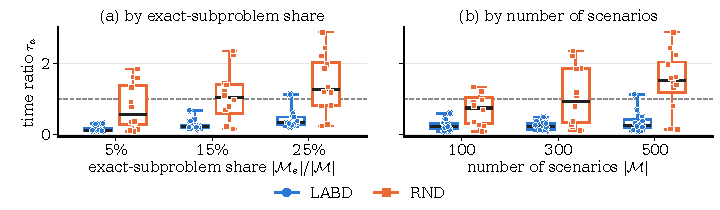
\includegraphics[width=\textwidth]{figures/fig_share.pdf}
\caption{Time ratio $\tau_a$ by exact-subproblem share (a) and by number of scenarios (b) for the configurations solved by Standard BD. The dashed line $\tau_a=1$ is Standard BD.}\label{fig:share}
\end{figure}



\begin{table}[!b]
\centering
\caption{Gap $\Delta_a$ (\%) relative to Standard BD on the configurations it solves (left) and on p20, where it reaches the time limit (right; over the configurations in which the method finds a feasible solution; negative is better). Opt.: $\Delta_a=0$; NS: no feasible solution.}\label{tab:gap}
\setlength{\tabcolsep}{5pt}
\begin{tabular}{lrrrr!{\vrule width 1pt}rrrr}
\toprule
& \multicolumn{4}{c!{\vrule width 1pt}}{\textbf{BD solved} ($n=36$)} & \multicolumn{4}{c}{\textbf{BD time limit} ($n=9$)}\\
\cmidrule(lr){2-5}\cmidrule(lr){6-9}
Method & Opt. & Mean & Med. & Max. & NS & Mean & Med. & Max.\\
\midrule
LABD & 34 & 0.08 & 0.00 & 1.56 & 0 & $-$1.86 & $-$2.35 & 2.38\\
RND  & 30 & 0.21 & 0.00 & 1.56 & 3 & 12.49 & 8.93 & 27.12\\
\bottomrule
\end{tabular}
\end{table}

\paragraph{Results.} Standard BD solves four of the five instances within the time limit for every number of scenarios, which gives 36 solved configurations per inexact method. Fig.~\ref{fig:share}(a) shows that LABD is markedly faster than Standard BD at every exact-subproblem share: it is about $4.6$ times faster in the median, and close to ten times faster when only $5\%$ of the subproblems are solved exactly. RND, which also solves only part of the subproblems exactly, gains much less: it is faster than Standard BD at the smallest share, close to it at $15\%$, and slower at $25\%$. The time ratio grows with the exact share, since each additional exact subproblem is solved in every cut-generation round, but for LABD this effort buys no better solutions: the smallest share already yields the optimal objective in almost every configuration. A small set of representative subproblems therefore carries most of the dual information needed to generate effective cuts, and the duals of the remaining subproblems can be inferred from it at negligible cost.

Fig.~\ref{fig:share}(b) shows how this advantage evolves with the size of the problem. As the number of scenarios grows from 100 to 500, the median time ratio of LABD remains between $0.21$ and $0.25$, whereas that of RND rises from $0.74$ to $1.53$. The benefit of LABD is thus maintained as the number of subproblems grows, while that of random selection vanishes.

Table~\ref{tab:gap} shows that the speed of LABD does not come at the expense of solution quality. LABD returns the optimal objective in 34 of the 36 solved configurations, against 30 for RND, and its mean gap is less than half that of RND. In the two configurations where LABD deviates, the gap remains below $1.6\%$.

The differences are sharper on p20, where Standard BD stops at the time limit with an optimality gap of $17$--$33\%$. LABD finds a feasible solution in all nine configurations and improves on the Standard BD incumbent in seven of them, by $1.86\%$ on average. RND returns no feasible solution in three configurations, because every integer candidate found during branch and bound was cut off by a violated Benders cut, and its solutions in the other six are on average $12.5\%$ worse than the Standard BD incumbent.

Since LABD and RND solve the same number of subproblems exactly, these differences reflect the representation-based selection and the certified prediction of LABD.

\section{Conclusion}\label{sec:conclusion}

We introduced Learning-Augmented Benders Decomposition (LABD), which solves a selected subset of subproblems exactly and predicts dual-feasible solutions for the rest. LABD learns representations of subproblem behavior from warm-up dual trajectories, uses them to select the exact subproblems, and certifies predicted duals by an explicit step from the mean of the current exact duals, so every cut remains valid; optimality-gap bounds separate the contribution of the exact subproblems from that of the prediction. On stochastic capacitated facility location instances solved by Standard BD, LABD is $4.6$ times faster than Standard BD in the median, and close to ten times faster when only $5\%$ of the subproblems are solved exactly, while returning the optimal objective in 34 of 36 configurations.

\label{end-of-main-body}% the page of this label must be <= 12
% ---------------------------- END OF MAIN BODY ----------------------------------

% Acknowledgements: IPCO requires disclosure of any AI/LLM use here.
% Do NOT acknowledge funders, advisors or supporters in the submitted version.
\begin{credits}
\subsubsection{\ackname}
The authors used a large language model to assist with editing the text and with writing and testing parts of the experimental code; all content was checked by the authors, who take full responsibility for it. Reviewers may upload this submission to a generative AI service.
\end{credits}

\bibliographystyle{splncs04}
\bibliography{references}

% ---------------------------- APPENDIX (no page limit; reviewed, not published) --
\appendix
\section{Proofs}\label{app:proofs}

\subsection{Proof of Theorem~\ref{thm:surrogate}}
\begin{proof}
Fix $\mathbf x\in\mathcal X$ and $m\in\mathcal M_p$. Every vector in the supremum of~\eqref{eq:surrogate} lies in $\mathcal D$, so by weak duality its objective at $\mathbf x$ is at most $Q_m(\mathbf x)$. Since $Q_m(\mathbf x)\ge0$, taking the supremum and the maximum with zero preserves the inequality, so $0\le\widehat Q_m(\mathbf x)\le Q_m(\mathbf x)$. The blocks in $\mathcal M_e$ enter $\widehat V$ exactly; multiplying by $\omega_m>0$ and adding $\mathbf c^\top\mathbf x$ gives~(i). For~(ii), optimality of $\widehat{\mathbf x}$ for $\widehat V$ and~(i) give $\widehat V(\widehat{\mathbf x})\le\widehat V(\mathbf x^*)\le V(\mathbf x^*)\le V(\widehat{\mathbf x})$. Subtracting $\widehat V(\widehat{\mathbf x})$ from the last term and cancelling the exactly represented blocks yields~\eqref{eq:surrogate-gap}.
\end{proof}

\subsection{Proof of Proposition~\ref{prop:repair}}
\begin{proof}
Along $\bar{\boldsymbol\lambda}+\gamma\mathbf d$, membership in $\mathcal D$ is equivalent to $\bar\lambda_j+\gamma d_j\ge0$ for all $j$ and $(\mathbf W^\top\bar{\boldsymbol\lambda})_\ell+q_\ell+\gamma(\mathbf W^\top\mathbf d)_\ell\ge0$ for all $\ell$. Because $\bar{\boldsymbol\lambda}\in\mathcal D$, every constant term is nonnegative, so each constraint with a nonnegative coefficient of $\gamma$ holds for all $\gamma\ge0$, and each constraint with a negative coefficient holds exactly for $\gamma$ up to the corresponding ratio in~\eqref{eq:gamma-max}. The feasible steps in $[0,1]$ therefore form the interval $[0,\gamma^{\max}]$. The objective $(\bar{\boldsymbol\lambda}+\gamma\mathbf d)^\top\mathbf g=\bar{\boldsymbol\lambda}^\top\mathbf g+\gamma\,\mathbf d^\top\mathbf g$ is affine in $\gamma$, so its maximum over the interval is attained at $\gamma^{\max}$ if $\mathbf d^\top\mathbf g>0$ and at $0$ otherwise (ties resolved toward the reference point).
\end{proof}

\subsection{Proof of Proposition~\ref{prop:certificate}}
\begin{proof}
Each $\boldsymbol\lambda_t(\mathbf x)$, $t\in\mathcal M_e$, is an extreme point of $\mathcal D$, and $\mathcal D$ is convex and does not depend on the block, so $\bar{\boldsymbol\lambda}(\mathbf x)\in\mathcal D$. Proposition~\ref{prop:repair} with this reference point shows that $\gamma_m(\mathbf x)\in\{0,\gamma_m^{\max}(\mathbf x)\}\subseteq[0,\gamma_m^{\max}(\mathbf x)]$ is a feasible step, so $\widehat{\boldsymbol\lambda}_m(\mathbf x)\in\mathcal D$. By~\eqref{eq:guard}, $\gamma_m(\mathbf x)\,\mathbf d_m(\mathbf x)^\top\mathbf g_m(\mathbf x)=\gamma_m^{\max}(\mathbf x)[\mathbf d_m(\mathbf x)^\top\mathbf g_m(\mathbf x)]_+\ge0$, which gives~\eqref{eq:improvement}.
\end{proof}

\subsection{Proof of Theorem~\ref{thm:performance}}
\begin{proof}
Fix $m\in\mathcal M_p$ and $\mathbf x\in\mathcal X$, suppress $\mathbf x$, and write $\mathbf g_m=\mathbf g_m(\mathbf x)$. The lower bound $0\le Q_m-\widehat Q_m$ is Theorem~\ref{thm:surrogate}. Let $\boldsymbol\lambda_m^\star\in\Lambda$ be optimal for block $m$, so $Q_m=\boldsymbol\lambda_m^{\star\top}\mathbf g_m$. For $t\in\mathcal M_e$, $\boldsymbol\lambda_t\in\Lambda$ is optimal for $\mathbf g_t$, hence $\boldsymbol\lambda_t^\top\mathbf g_t\ge\boldsymbol\lambda_m^{\star\top}\mathbf g_t$ and
\[
\boldsymbol\lambda_m^{\star\top}\mathbf g_m-\boldsymbol\lambda_t^\top\mathbf g_m
\le\boldsymbol\lambda_m^{\star\top}\mathbf g_m-\boldsymbol\lambda_m^{\star\top}\mathbf g_t+\boldsymbol\lambda_t^\top\mathbf g_t-\boldsymbol\lambda_t^\top\mathbf g_m
=(\boldsymbol\lambda_m^\star-\boldsymbol\lambda_t)^\top(\mathbf g_m-\mathbf g_t)
\le\Delta_\Lambda\|\mathbf g_m-\mathbf g_t\|_2,
\]
by the Cauchy--Schwarz inequality and~\eqref{eq:diameter}. Averaging over $t\in\mathcal M_e$ gives $Q_m-\bar{\boldsymbol\lambda}^\top\mathbf g_m\le\frac{\Delta_\Lambda}{p}\sum_{t\in\mathcal M_e}\|\mathbf g_m-\mathbf g_t\|_2$. The certified prediction at $\mathbf x$ is one of the vectors in the supremum defining $\widehat Q_m(\mathbf x)$, so by~\eqref{eq:improvement}
\[
\widehat Q_m\ge\widehat{\boldsymbol\lambda}_m^\top\mathbf g_m=\bar{\boldsymbol\lambda}^\top\mathbf g_m+\gamma_m\,\mathbf d_m^\top\mathbf g_m .
\]
Combining the two displays proves~\eqref{eq:recourse-bound}. Inserting~\eqref{eq:recourse-bound} at $\widehat{\mathbf x}$ into~\eqref{eq:surrogate-gap} and summing with weights $\omega_m>0$ proves~\eqref{eq:gap-bound}.
\end{proof}

\section{Multi-cut Benders Decomposition and the LABD Master Problem}\label{app:classical-bd}

With $\boldsymbol\eta=(\eta_m)_{m\in\mathcal M}$, the exact multi-cut reformulation of~\eqref{eq:two-stage} is
\begin{equation}\label{eq:full-master}
\min_{\mathbf x\in\mathcal X,\ \boldsymbol\eta\ge\mathbf 0}\ \mathbf c^\top\mathbf x+\sum_{m\in\mathcal M}\omega_m\eta_m
\quad\text{s.t.}\quad \eta_m\ge\boldsymbol\lambda^\top\mathbf g_m(\mathbf x),\qquad m\in\mathcal M,\ \boldsymbol\lambda\in\Lambda .
\end{equation}
Under relatively complete recourse no feasibility cuts are needed~\cite{birge2006introduction}. Algorithm~\ref{alg:classical-bd} states the classical multi-cut method. The restricted master keeps, for each subproblem, only the cuts generated so far; at iteration $k$ its value gives the lower bound $LB^k$, and exact evaluation of all subproblems at $\mathbf x^k$ gives a candidate upper bound.

\begin{algorithm}[h]
\caption{Classical multi-cut Benders decomposition}\label{alg:classical-bd}
\begin{algorithmic}[1]
\Require optimality-gap tolerance $\epsilon>0$
\State $\Lambda_m\gets\varnothing$ for all $m\in\mathcal M$; $UB\gets+\infty$; $k\gets0$
\Loop
\State $k\gets k+1$; solve $\min\{\mathbf c^\top\mathbf x+\sum_m\omega_m\eta_m:\ \eta_m\ge\boldsymbol\lambda^\top\mathbf g_m(\mathbf x)\ (\boldsymbol\lambda\in\Lambda_m,\ m\in\mathcal M),\ \boldsymbol\eta\ge\mathbf 0,\ \mathbf x\in\mathcal X\}$
\State let $(\mathbf x^k,\boldsymbol\eta^k)$ be optimal and $LB^k\gets\mathbf c^\top\mathbf x^k+\sum_m\omega_m\eta_m^k$
\For{$m\in\mathcal M$}
\State solve~\eqref{eq:dual-subproblem} at $\mathbf x^k$ and obtain $\boldsymbol\lambda_m^k\in\Lambda$
\If{$\eta_m^k<(\boldsymbol\lambda_m^k)^\top\mathbf g_m(\mathbf x^k)$} $\Lambda_m\gets\Lambda_m\cup\{\boldsymbol\lambda_m^k\}$ \EndIf
\EndFor
\If{$V(\mathbf x^k)<UB$} $UB\gets V(\mathbf x^k)$; $\bar{\mathbf x}\gets\mathbf x^k$ \EndIf
\If{$UB-LB^k<\epsilon$} \Return $\bar{\mathbf x}$, $UB$ \EndIf
\EndLoop
\end{algorithmic}
\end{algorithm}

In the single-tree implementation used here, the master is solved once by branch and bound, and the cut-generation step of Algorithm~\ref{alg:classical-bd} is carried out in solver callbacks at LP-relaxation and integer-feasible solutions~\cite{rostami2022single,rostami2023convex}. LABD runs the same scheme on the formulation~\eqref{model:labd}: in the cut-generation step, subproblems $t\in\mathcal M_e$ are solved exactly, and subproblems $m\in\mathcal M_p$ receive the certified prediction~\eqref{eq:certified}. Since~\eqref{model:labd} is equivalent to $\min_{\mathbf x\in\mathcal X}\widehat V(\mathbf x;\pi_{\boldsymbol\theta})$ (Section~\ref{subsec:labd}), its restricted master value bounds $\min_{\mathbf x}\widehat V$ from below, and the final solution is re-evaluated exactly to obtain $V(\widehat{\mathbf x})$.

\section{Block Representations from Warm-up Duals}\label{app:representation}

Given $\boldsymbol\Omega$ in~\eqref{eq:omega}, each discrepancy is turned into an affinity $a_{ij}:=\exp(-\Omega_{ij}/\tau)$ for $i\ne j$ and $a_{ii}:=0$, with temperature $\tau>0$, and into transition probabilities $\rho_{ij}:=a_{ij}/\sum_{l\ne i}a_{il}$. From each block we generate $n_{\mathrm{walk}}$ random walks of length $\ell_{\mathrm{walk}}$ with these probabilities, and train a skip-gram model with window $w$ and dimension $d$ on the walk corpus~\cite{perozzi2014deepwalk,mikolov2013distributed}. The embedding of block $m$ is its representation $\mathbf z_m$. When a block has several optimal duals during warm-up, the representation can depend on which one the solver returns; we use the solver's choice under fixed settings, and a deterministic tie-breaking rule can be imposed when exact reproducibility is required. In all experiments we use $|\mathcal K_0|=5$ warm-up rounds, $\varepsilon_{\mathrm{stab}}=10^{-12}$, $\tau=1$, $n_{\mathrm{walk}}=2$, $\ell_{\mathrm{walk}}=5$, $w=5$ and $d=3$ for the representation, and $q=3$ and $\beta_z=\beta_g=10^{-3}$ for the mapping of Section~\ref{subsec:direct}. The $p$-median problem~\eqref{eq:pmedian} is solved by a deterministic build-and-swap heuristic with a 300-second limit.

\section{Experimental Details}\label{app:experiments}

\subsection{SCFLP Formulation and Benders Reformulation}\label{app:scflp}

Let $\mathcal J$ be the set of candidate facilities and $\mathcal I$ the set of customers. Opening facility $j\in\mathcal J$ incurs a fixed cost $f_j$ and provides capacity $u_j$; the binary variable $x_j$ equals one if facility $j$ is opened. Serving one unit of demand of customer $i\in\mathcal I$ from facility $j$ costs $c_{ij}$. Let $\mathcal M$ be the set of equally likely demand scenarios, $d_{i,m}$ the demand of customer $i$ in scenario $m$, and $y_{ij}^m$ the amount supplied from $j$ to $i$ in scenario $m$. The sample average approximation of the SCFLP is
\begin{subequations}\label{model:scflp-saa}
\begin{align}
\min_{\mathbf x,\{\mathbf y^m\}}\quad & \sum_{j\in\mathcal J}f_jx_j+\frac{1}{|\mathcal M|}\sum_{m\in\mathcal M}\sum_{i\in\mathcal I}\sum_{j\in\mathcal J}c_{ij}y_{ij}^m\\
\text{s.t.}\quad & \sum_{j\in\mathcal J}u_jx_j\ge\max_{m\in\mathcal M}\sum_{i\in\mathcal I}d_{i,m}, \label{model:scflp-saa:rcr}\\
& \sum_{j\in\mathcal J}y_{ij}^m\ge d_{i,m}, && i\in\mathcal I,\ m\in\mathcal M, \label{model:scflp-saa:demand}\\
& \sum_{i\in\mathcal I}y_{ij}^m\le u_jx_j, && j\in\mathcal J,\ m\in\mathcal M, \label{model:scflp-saa:capacity}\\
& y_{ij}^m\ge0,\quad x_j\in\{0,1\}, && i\in\mathcal I,\ j\in\mathcal J,\ m\in\mathcal M.
\end{align}
\end{subequations}
Constraints~\eqref{model:scflp-saa:demand}--\eqref{model:scflp-saa:capacity} enforce demand satisfaction and facility capacities in every scenario. Because every customer can be served from every open facility, constraint~\eqref{model:scflp-saa:rcr} guarantees enough aggregate capacity for the largest sampled total demand and hence relatively complete recourse.

\paragraph{Scenario subproblems.} For fixed $\mathbf x$, \eqref{model:scflp-saa} separates into the first-stage problem $\min\{\sum_jf_jx_j+\frac{1}{|\mathcal M|}\sum_mQ_m(\mathbf x):\ \eqref{model:scflp-saa:rcr},\ \mathbf x\in\{0,1\}^{|\mathcal J|}\}$ and the scenario subproblems
\begin{subequations}\label{model:scflp-sub}
\begin{align}
Q_m(\mathbf x):=\min_{\mathbf y^m\ge\mathbf 0}\quad & \sum_{i\in\mathcal I}\sum_{j\in\mathcal J}c_{ij}y_{ij}^m\\
\text{s.t.}\quad & \sum_{j\in\mathcal J}y_{ij}^m\ge d_{i,m}, && i\in\mathcal I,\\
& \sum_{i\in\mathcal I}y_{ij}^m\le u_jx_j, && j\in\mathcal J.
\end{align}
\end{subequations}

\paragraph{Dual representation and optimality cuts.} Let $\mu_i\ge0$ and $\nu_j\ge0$ be the duals of the demand and capacity constraints of~\eqref{model:scflp-sub}, and
\[
\mathcal D_{\mathrm F}:=\bigl\{(\boldsymbol\mu,\boldsymbol\nu)\ge\mathbf 0:\ \mu_i-\nu_j\le c_{ij},\ i\in\mathcal I,\ j\in\mathcal J\bigr\}.
\]
Then
\begin{equation}\label{model:scflp-dual}
Q_m(\mathbf x)=\max_{(\boldsymbol\mu,\boldsymbol\nu)\in\mathcal D_{\mathrm F}}\Bigl\{\sum_{i\in\mathcal I}d_{i,m}\mu_i-\sum_{j\in\mathcal J}u_jx_j\nu_j\Bigr\},
\end{equation}
and any $(\boldsymbol\mu,\boldsymbol\nu)\in\mathcal D_{\mathrm F}$, exact or predicted, gives the valid optimality cut
\begin{equation}\label{eq:scflp-cut}
\eta_m\ge\sum_{i\in\mathcal I}d_{i,m}\mu_i-\sum_{j\in\mathcal J}u_jx_j\nu_j .
\end{equation}
In the notation of Section~\ref{sec:setting}, $\boldsymbol\lambda=(\boldsymbol\mu,\boldsymbol\nu)$, $\mathcal D=\mathcal D_{\mathrm F}$ and $\mathbf g_m(\mathbf x)=(\mathbf d_m,\,-(u_jx_j)_{j\in\mathcal J})$, where $\mathbf d_m:=(d_{i,m})_{i\in\mathcal I}$. Only the demands vary with $m$, so $\mathbf T_m=\mathbf T$ for all $m$, and $\mathcal D_{\mathrm F}$ contains $\mathbf 0$ since $c_{ij}\ge0$. The Benders master problem consists of the first-stage objective with $\frac{1}{|\mathcal M|}\sum_m\eta_m$, constraint~\eqref{model:scflp-saa:rcr}, $\eta_m\ge0$ and the cuts~\eqref{eq:scflp-cut}; Standard BD generates them from optimal solutions of~\eqref{model:scflp-dual} for all $m$, and LABD from exact duals for $m\in\mathcal M_e$ and certified predictions for $m\in\mathcal M_p$. Because of~\eqref{model:scflp-saa:rcr}, only optimality cuts are needed.

\subsection{Instances and Data Generation}\label{app:instances}

We use the deterministic instances p4, p5, p10, p20 and p50 of~\cite{holmberg1999exact}. Instances p4, p5 and p10 have 50 customers and 10 candidate facilities, p20 has 50 customers and 20 facilities, and p50 has 100 customers and 10 facilities. The Holmberg data give the cost of serving the whole demand of customer $i$ from facility $j$; we use the corresponding unit cost $c_{ij}/\bar d_i$.

Each instance is extended to $|\mathcal M|\in\{100,300,500\}$ scenarios with weight $\omega_m=1/|\mathcal M|$. Adapting the demand-generation procedure of~\cite{bodur2017strengthened}, let $\bar d_i$ be the baseline demand of customer $i$. We draw $\sigma_i\sim\operatorname{Uniform}(0.1\bar d_i,\,0.3\bar d_i)$ and set $d_{i,m}=\max\{0,D_{i,m}\}$ with $D_{i,m}\sim\mathcal N(\bar d_i,\sigma_i^2)$. The demands are scaled where necessary to satisfy the capacity condition~\eqref{model:scflp-saa:rcr}.

\subsection{Computational Implementation}\label{app:implementation}

All methods use the same single-tree multi-cut Benders implementation (Appendix~\ref{app:classical-bd}): the master MIP is processed in a single branch-and-bound tree, and cuts are added in callbacks at LP-relaxation and integer-feasible solutions. The $p$-median problem~\eqref{eq:pmedian} is approximated by a deterministic build-and-swap heuristic. The mapping is linear with no intercept, $f_{\boldsymbol\theta}(\mathbf z,\mathbf s)=\boldsymbol\Theta_z\mathbf z+\boldsymbol\Theta_g\mathbf s$, and is trained in~\eqref{model:training} with the squared loss and the ridge penalty $\mathcal R(\boldsymbol\theta)=\beta_z\|\boldsymbol\Theta_z\|_F^2+\beta_g\|\boldsymbol\Theta_g\|_F^2$. The state map $\phi_g$ projects $\mathbf g_m(\mathbf x)$, without centring or scaling, onto the leading $q$ right singular vectors of the matrix of warm-up states. LABD uses certified predictions for its prediction subproblems at both callback locations, and RND uses its averaged duals at both. Hyperparameter values are listed in Appendix~\ref{app:representation}.

\subsection{Termination and Evaluation Conventions}\label{app:conventions}

A configuration is \emph{solved by Standard BD} when Standard BD terminates within the three-hour limit after meeting the $0.1\%$ optimality tolerance; otherwise it is \emph{not solved by Standard BD}. Meeting the tolerance does not require a zero optimality gap. For every returned first-stage solution, the objective $V_a$ used in $\Delta_a$ is computed by fixing that solution and solving all scenario subproblems exactly. For configurations solved by Standard BD, $\Delta_a$ compares $V_a$ with the objective of the completed Standard BD run; for the others, it compares the best feasible solutions returned within the common time limit and is not a certified optimality gap. Recorded runtimes can slightly exceed three hours, because the solver may finish its current work before returning after the time limit.

\clearpage
\section{Background for Discussion (not part of the submission)}\label{app:meeting}

This section collects implementation details and run diagnostics for discussion among the authors. Unless stated otherwise, the statistics are medians over the 36 configurations solved by Standard BD (instances p4, p5, p10 and p50 with 100, 300 and 500 scenarios).

\subsection{Gurobi Settings}\label{app:gurobi}

Table~\ref{tab:gurobi} lists the Gurobi~12.0.0 parameters that matter for single-tree Benders, their meaning, the Gurobi default, typical choices in the literature, and our setting. Parameters not listed are at their defaults (e.g., \texttt{Presolve}, \texttt{MIPFocus}, \texttt{Cuts}, \texttt{Heuristics}=0.05, \texttt{Seed}=0, \texttt{FeasibilityTol}=\texttt{OptimalityTol}=$10^{-6}$, \texttt{IntFeasTol}=$10^{-5}$). The scenario subproblems are LPs solved with default settings and \texttt{OutputFlag}=0; the master problem prints its log.

\begin{table}[h]
\centering
\caption{Gurobi parameters of the master MIP.}\label{tab:gurobi}
\scriptsize
\setlength{\tabcolsep}{3pt}
\begin{tabular}{p{2.1cm}p{4.3cm}p{1.2cm}p{2.2cm}p{1.6cm}}
\toprule
Parameter & Meaning & Default & Common choices & Ours\\
\midrule
\texttt{LazyConstraints} & must be 1 to add constraints with \texttt{cbLazy} at integer candidates (\texttt{MIPSOL}); disables reductions that could cut off solutions & 0 & 1 in every single-tree Benders code & 1\\
\texttt{MIPGap} & stop when $(UB-LB)/|UB|$ is below this value & $10^{-4}$ & $10^{-4}$ (default), $10^{-3}$ or $10^{-2}$ in Benders studies & $10^{-3}$\\
\texttt{TimeLimit} & wall-clock limit in seconds & $\infty$ & 1--3 h; 3 h (10\,800 s) is frequent & 10\,800\\
\texttt{Threads} & number of threads (0 = all cores) & 0 & equal to the allocated cores & 16 (via \texttt{gurobi.env})\\
\texttt{PreCrush} & lets presolve translate user cuts added with \texttt{cbCut} at \texttt{MIPNODE}; Gurobi asks for 1 when adding user cuts & 0 & 1 when \texttt{cbCut} is used & 0 (not set)\\
\texttt{OutputFlag} & solver log on/off & 1 & 1 for the master, 0 for subproblems & 1 / 0\\
\texttt{Method} & LP algorithm ($-1$ automatic, 0 primal, 1 dual simplex, 2 barrier) & $-1$ & dual simplex for repeated subproblem LPs & $-1$\\
\bottomrule
\end{tabular}
\end{table}

Cuts are added at integer candidates with \texttt{cbLazy} (callback \texttt{MIPSOL}) and at fractional nodes with \texttt{cbCut} (callback \texttt{MIPNODE}, only when the node LP is optimal). The Gurobi logs report all retained Benders cuts as ``Lazy constraints'' and no ``User'' cuts; whether the \texttt{cbCut} cuts are used without \texttt{PreCrush}=1 is worth checking, because it affects all methods equally.

\subsection{Data Generation}\label{app:datagen}

The scenario files are produced by \texttt{SCFLP\_data\_generation\_version4.py} (method \texttt{merve\_with\_covariate\_with\_random\_demand\_capacity}, NumPy \texttt{default\_rng} with seed 42 for every file), starting from the corrected reading of the Holmberg instances (capacity and fixed cost per facility, unit cost $c_{ij}/\bar d_i$).
\begin{enumerate}
\item \emph{Capacity scenarios.} For each facility, $\sigma^u_j\sim U(0.1u_j,0.3u_j)$; scenario 1 keeps $u_j$, and scenarios $2,\dots,S$ draw $u_{j,m}\sim\mathcal N(u_j,(\sigma^u_j)^2)$, clipped at zero.
\item \emph{Demand scenarios.} For each customer, $\sigma_i\sim U(0.1\bar d_i,0.3\bar d_i)$, and $d_{i,m}=\max\{0,D_{i,m}\}$ with $D_{i,m}\sim\mathcal N(\bar d_i,\sigma_i^2)$. If $\sum_i d_{i,m}$ exceeds the total capacity of scenario $m$, all demands of the scenario are multiplied by 0.9 until it does not.
\item \emph{Covariates.} The scenario matrix $[\mathbf d_m,\mathbf u_m]_{m}$ is centred, and the first six left singular vectors of its SVD give six PCA covariates per scenario.
\item \emph{Predictability diagnostics.} For each customer (and facility), the demand (capacity) is predicted from the covariates with linear regression, $k$-NN ($k=2$), $k$-means clustering (up to 10 clusters) and a regression tree on an 80/20 split; the training $R^2$, test MSE and test MAPE are written to the \texttt{\# Diagnostics} block of the file.
\end{enumerate}
The runs use \texttt{use\_stochastic\_capacity}=False and \texttt{use\_covariates}=\texttt{features\_only} (VERIFIED in all 105 solution logs): the stored capacity scenarios and covariates are not used by the solver or by LABD, the second stage uses the base capacities $u_j$, so $\mathbf T_m=\mathbf T$, and relatively complete recourse is enforced by the master constraint $\sum_ju_jx_j\ge\max_m\sum_id_{i,m}$.

\subsection{What Happens Inside the Runs}\label{app:runstats}

Table~\ref{tab:runstats} and Fig.~\ref{fig:diag} report how the solve proceeds. A \emph{callback} is one cut-generation round, at an integer candidate or at a fractional node. \emph{Integer candidates} are the \texttt{MIPSOL} callbacks, i.e., integer master solutions submitted to the callback, most of which are cut off. \emph{Cuts generated} counts the cuts built from exact and from predicted (or averaged) duals; \emph{cuts in master} is the number of lazy constraints Gurobi keeps at the end.

\begin{table}[h]
\centering
\caption{Median run statistics on the configurations solved by Standard BD (times in seconds).}\label{tab:runstats}
\scriptsize
\setlength{\tabcolsep}{3pt}
\begin{tabular}{lrrrrrrrrr}
\toprule
Method & Time & Warm-up & $p$-median & Callbacks & B\&B nodes & Int.\ cand. & \multicolumn{2}{c}{Cuts generated} & Cuts in master\\
\cmidrule(lr){8-9}
 & & & & & & & exact & predicted & \\
\midrule
Standard BD & 762 & -- & -- & 291 & 298 & 76 & 71\,615 & -- & 15\,651\\
LABD 5\% & 82 & 15 & 0.5 & 280 & 300 & 85 & 4\,694 & 70\,170 & 18\,865\\
LABD 15\% & 156 & 14 & 4.6 & 293 & 304 & 77 & 11\,060 & 57\,006 & 15\,508\\
LABD 25\% & 233 & 14 & 8.2 & 271 & 275 & 81 & 18\,166 & 51\,499 & 16\,565\\
RND 5\% & 230 & -- & -- & 1\,275 & 923 & 484 & 11\,354 & 110\,211 & 40\,218\\
RND 15\% & 416 & -- & -- & 1\,110 & 897 & 390 & 26\,487 & 114\,182 & 41\,609\\
RND 25\% & 518 & -- & -- & 978 & 748 & 378 & 35\,088 & 82\,169 & 34\,931\\
\bottomrule
\end{tabular}
\end{table}

\begin{figure}[h]
\centering
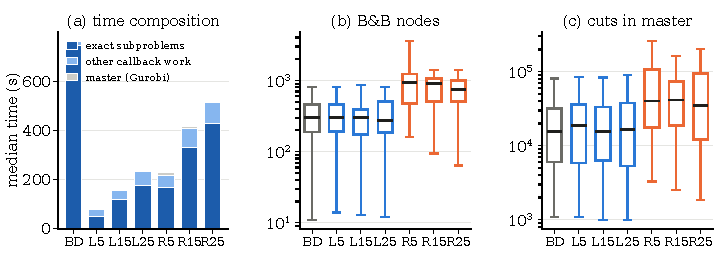
\includegraphics[width=\textwidth]{figures/fig_diag.pdf}
\caption{(a) Median solution time split into exact subproblem solves, other callback work (prediction, certification, selection, cut construction) and the master MIP. (b) Branch-and-bound nodes and (c) Benders cuts retained in the master, log scale. BD: Standard BD; L5--L25: LABD with 5--25\% exact share; R5--R25: RND.}\label{fig:diag}
\end{figure}

Three observations follow.
\begin{itemize}
\item \emph{LABD follows the same search as Standard BD.} It needs about the same number of callbacks (about 280 versus 291), nodes and integer candidates, and keeps a similar number of cuts. Each callback is cheaper because only the $p$ representative subproblems are solved exactly: exact subproblem time drops from about 743~s to 49--201~s.
\item \emph{RND searches much more.} With averaged duals of random subproblems, its cuts are weaker: it needs 3--4 times more callbacks and 2.5--3 times more nodes, submits about five times more integer candidates (most cut off), and keeps 2--3 times more cuts in the master. This is why it is not faster despite solving the same number of subproblems exactly.
\item \emph{Fixed costs of LABD.} Warm-up takes about 15~s (all subproblems solved exactly for five rounds), and the $p$-median selection grows with the share (median 0.5~s at 5\%, 8~s at 25\%, up to 210~s on p4 with 500 scenarios). Training, prediction, certification and the guard together take a few seconds. About 73\% of the raw predictions are infeasible and are certified.
\end{itemize}

\subsection{Bounds over Time}\label{app:lbub}

Fig.~\ref{fig:lbub} plots the lower bound (LB, best bound of the master) and the upper bound (UB, incumbent of the master) recorded in every callback, together with the master gap $(UB-LB)/UB$, for a typical instance (p4, 500 scenarios) and for p10 with 300 scenarios. For Standard BD both bounds refer to the true problem. For LABD and RND they refer to the \emph{surrogate} master built with predicted or averaged cuts: the run stops when the surrogate gap is below $0.1\%$, and the returned solution is then evaluated exactly. The dotted line is the optimal objective.

\begin{figure}[h]
\centering
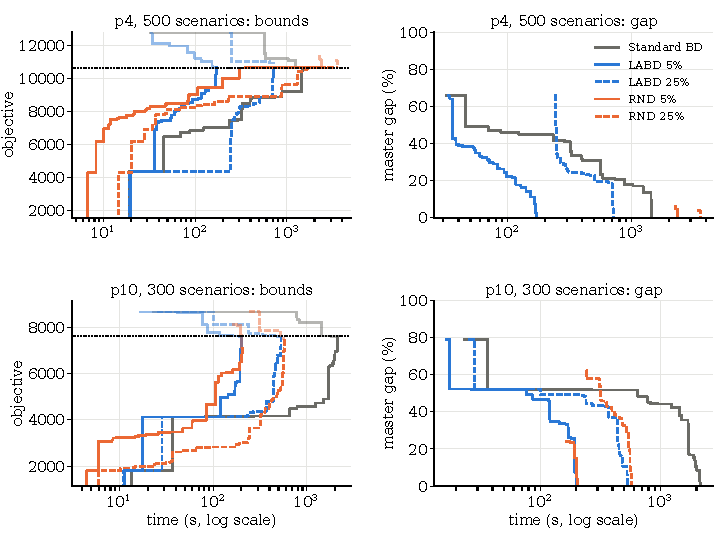
\includegraphics[width=\textwidth]{figures/fig_lbub.pdf}
\caption{Master lower bound (rising curves) and upper bound (lighter falling curves), and master gap, over time. Solid: 5\% exact share; dashed: 25\%.}\label{fig:lbub}
\end{figure}

\begin{itemize}
\item On p4, LABD closes the gap in 171~s at 5\% and 717~s at 25\%, against 1\,465~s for Standard BD. Its bounds follow the same pattern as those of Standard BD, compressed in time.
\item RND raises its lower bound quickly, but it finds no incumbent for a long time: Gurobi keeps proposing integer solutions and the callback keeps cutting them off with new averaged cuts. On p4 its first incumbent appears only after about 2\,265~s at 5\% (Standard BD and LABD have one after about 30~s), which is why its total time exceeds that of Standard BD.
\item On p10 with 300 scenarios, RND at 5\% is as fast as LABD, but its surrogate stops at a bound of 7\,093, far below the optimum 7\,611: its averaged cuts underestimate the recourse, and the returned solution is $1.56\%$ worse than optimal. LABD stops at 7\,603, just below the optimum, and returns the optimal solution.
\end{itemize}

\subsection{Reading a Gurobi Log}\label{app:gurobilog}

The folder \texttt{logs/} of this repository contains the Gurobi logs of the master problem for p10 with 300 scenarios (Standard BD, LABD 5\%, RND 5\%). The main parts of the Standard BD log are as follows.

\begin{enumerate}
\item \emph{Header.} \texttt{Read parameters from file gurobi.env} sets \texttt{Threads}=16; then \texttt{LazyConstraints}, \texttt{MIPGap} and \texttt{TimeLimit} are set by the code, and the block ``Non-default parameters'' confirms them.
\item \emph{Model.} \texttt{Optimize a model with 2 rows, 310 columns}: the master starts with only the capacity constraint (plus one constraint presolve removes), 10 binary facility variables and 300 continuous recourse variables $\eta_m$; all Benders cuts are added later through the callback.
\item \emph{Root relaxation.} Objective 1\,800: without any cut the $\eta_m$ can be zero, so the first bound is the LP bound on the fixed costs alone. Benders cuts raise it during the search.
\item \emph{Node log.} Each line reports explored and unexplored nodes, the node objective and depth, the number of fractional variables (\texttt{IntInf}), the incumbent, the best bound (\texttt{BestBd}), the gap, simplex iterations per node and elapsed time. A line starting with \texttt{H} is an incumbent found by a heuristic, and \texttt{*} an incumbent found at a node; both must first survive the lazy-cut check in the callback.
\item \emph{Cut summary.} \texttt{Cutting planes: Lazy constraints: 44701} is the number of Benders cuts retained in the master. No ``User'' cuts are listed, although the trace records about 143\,000 cuts submitted with \texttt{cbCut} at fractional nodes; this supports the \texttt{PreCrush} question in Appendix~\ref{app:gurobi}.
\item \emph{Termination.} \texttt{Explored 745 nodes \ldots\ in 2149.39 seconds}, \texttt{Optimal solution found (tolerance 1.00e-03)}, best objective and bound 7\,611.37. The last line, \texttt{User-callback calls 2694, time in user-callback 2138.32 sec}, shows that 99.5\% of the time is spent in the callback, i.e., in solving subproblems and building cuts; the master MIP itself takes about 11~s.
\end{enumerate}

The LABD and RND logs read the same way. Their ``best objective'' is the surrogate value (7\,603 for LABD, 7\,093 for RND), not $V(\widehat{\mathbf x})$; LABD spends 195 of its 201~s in the callback, and RND 198 of 205~s.

\section{Additional Convergence and Prediction Diagnostics}\label{app:trace-audit}

This section examines what happens \emph{during} the computations, beyond the total running times and returned objectives in Section~\ref{sec:results}. It uses the event-level traces supplied with the IPCO experiments and the matched summary in the IPCO coding repository (\path{results/ipco_20261108/}). The comparison is restricted to the direct-ridge, $p$-median, start-at-the-mean variant \path{PARAMETRIC_DIRECT_RIDGE_PMEDIAN_MEAN_V0} (LABD), Standard BD, and random selection with dual averaging (RND). The later clipped/shrunken-anchor and exact-fallback variants are \emph{not} pooled with these runs.

\paragraph{Trace coverage and measurement.}
For each of the five instances p4, p5, p10, p20, and p50 and each scenario count $S\in\{100,300,500\}$, there is one Standard BD run, three RND runs, and three LABD runs at exact-subproblem shares $5\%$, $15\%$, and $25\%$: 105 matched runs in total. The 100- and 300-scenario traces come from the corresponding \path{ipco_full100_pmedian_v0} and \path{ipco_full300_pmedian_v0} roots; the 500-scenario Standard BD/RND traces come from \path{ipco_full_pmedian}, and its LABD traces from \path{ipco_cmp_pmedian_v0}. The longer dated root names and job numbers are recorded in the results README. Seventeen additional traces in the supplied archive belong to earlier or different versions and are excluded. All 105 selected CSV traces use the \texttt{gurobi\_master\_v3\_events} schema, terminate with a \texttt{solver\_final} event, and report no inconsistent recorded bound pairs.

A \emph{cut-generation round} is an observed \texttt{solver\_iteration\_start} event, not every internal Gurobi callback. The \emph{first-incumbent time} $t_{\mathrm{inc}}$ is the first event at which the recorded \emph{master} upper bound is finite. The trace duration $T$ is the elapsed time at \texttt{solver\_final}. The reported node count is Gurobi's explored branch-and-bound nodes at that event. These measurements concern the master solved by each method: for LABD and RND its bounds are those of the surrogate model, not bounds on the true objective unless independently verified. Submitted lazy/user cuts are submission counts and must not be interpreted as accepted or distinct cuts.

\subsection{Time to a Master Incumbent and Search Effort}\label{app:trace-incumbents}

Table~\ref{tab:trace-incumbents} uses the four instance families for which Standard BD terminates within the time limit (p4, p5, p10, and p50). For each scenario count, the Standard BD row is the median over four runs and the LABD/RND rows are medians over twelve runs (four instances times three exact shares). Each column is summarized separately; ratios of column medians need not equal the median of run-level ratios.

\begin{table}[ht]
\centering
\caption{Master-incumbent appearance and search effort, excluding p20 (medians from event traces). The time fraction is computed within each run before taking its median.}
\label{tab:trace-incumbents}
\scriptsize
\setlength{\tabcolsep}{4pt}
\begin{tabular}{rr r r r r}
\toprule
$S$ & Method & $t_{\mathrm{inc}}$ (s) & $100t_{\mathrm{inc}}/T$ (\%) & Cut rounds & B\&B nodes\\
\midrule
100 & BD   & 6.6  & 2.0  & 311 & 323\\
100 & LABD & 6.5  & 9.7  & 263 & 296\\
100 & RND  & 49.9 & 86.7 & 903 & 771\\
\midrule
300 & BD   & 25.7  & 2.3  & 274 & 287\\
300 & LABD & 23.4  & 13.4 & 289 & 310\\
300 & RND  & 170.2 & 93.3 & 971 & 822\\
\midrule
500 & BD   & 43.3  & 2.3  & 279 & 297\\
500 & LABD & 84.3  & 23.4 & 285 & 290\\
500 & RND  & 482.5 & 89.4 & 1750 & 1050\\
\bottomrule
\end{tabular}
\end{table}

LABD generally reaches a first master incumbent on a time scale comparable to Standard BD, and it needs a similar number of cut-generation rounds and explored nodes. RND typically spends most of its run before its first incumbent and explores substantially more of the tree. Across the 36 matched configurations on these four instances, the median ratios to the corresponding Standard BD run are $1.01$ for LABD versus $5.51$ for RND in cut-generation rounds, and $1.01$ versus $3.63$ in explored nodes. These are \emph{observed search patterns}, not a proof that one method's cuts dominate another's everywhere.

\subsection{The Difficult p20 Instance}\label{app:trace-p20}

Standard BD reaches the time limit on p20 at all three scenario counts. Table~\ref{tab:trace-p20} isolates the $15\%$ exact-share runs, for which both inexact methods returned a feasible first-stage solution at every size. The signed objective difference $\Delta$ is defined in~\eqref{eq:metrics}; since BD is time-limited here, a negative value means improvement over its \emph{incumbent}, not proven optimality. The BD gap is its final master optimality gap.

\begin{table}[ht]
\centering
\caption{p20 at the $15\%$ exact share: time to the first master incumbent and exactly evaluated objective relative to time-limited Standard BD.}
\label{tab:trace-p20}
\scriptsize
\setlength{\tabcolsep}{4pt}
\begin{tabular}{r r r r r r}
\toprule
$S$ & BD gap (\%) & LABD $t_{\mathrm{inc}}$ (s) & RND $t_{\mathrm{inc}}$ (s) & $\Delta_{\mathrm{LABD}}$ (\%) & $\Delta_{\mathrm{RND}}$ (\%)\\
\midrule
100 & 16.8 & 7.5  & 1\,730 & $-3.11$ & $+1.30$\\
300 & 29.8 & 28.7 & 3\,670 & $-3.48$ & $+27.12$\\
500 & 33.1 & 99.7 & 9\,009 & $-2.35$ & $+3.10$\\
\bottomrule
\end{tabular}
\end{table}

The slow appearance of a master incumbent under RND becomes especially pronounced on p20. At $S=500$, the $15\%$ RND run first records an incumbent after roughly 9\,009~s, whereas LABD does so after 100~s. The RND runs with $5\%$ exact scenarios at $S=300$, and with $5\%$ and $25\%$ at $S=500$, never record a master incumbent and have no exactly evaluated returned solution. LABD returns one in all nine p20 configurations; at $S=100$ its $5\%$ and $15\%$ runs also satisfy the solver's surrogate stopping criterion before the limit. None of these observations establishes that the true p20 optimum has been found.

\subsection{Master Convergence versus Original-Problem Quality}\label{app:trace-gaps}

A small or zero final master gap is \emph{not} a guarantee that the returned first-stage solution is optimal for the original stochastic program. For example, on p10 with 300 scenarios and $15\%$ exact solves, the LABD trace ends with a surrogate master lower and upper bound both near $6\,346.79$, while full exact evaluation gives $V(\widehat{\mathbf x})=7\,730.24$. The matched Standard BD objective is $7\,611.37$, so the returned original objective is $1.56\%$ higher even though the surrogate master has closed its own gap. This is why Section~\ref{sec:results} reports the original-objective difference $\Delta$ separately from the solver stopping criterion. The final evaluation and the valid surrogate lower bound provide an original-problem certificate, but that certificate can be much looser than the master stopping tolerance.

\subsection{Did the Direct Ridge Correction Affect the Cuts?}\label{app:trace-guard}

An additional audit uses the per-run \texttt{parametric\_objective\_guard\_checks} and \texttt{parametric\_objective\_guard\_accepted} counters in the coding repository's matched result CSV. The V0 rule begins feasibility restoration from the \emph{unshrunk mean} of the currently solved exact duals and accepts a repaired prediction only when its dual objective improves over that mean at the generating first-stage point. Table~\ref{tab:trace-guard} reports every LABD run in the same matched experiment set.

\begin{table}[ht]
\centering
\caption{Direct-ridge guard audit. Median $\tau$ is calculated only on the twelve matched configurations per scenario count where Standard BD finishes.}
\label{tab:trace-guard}
\scriptsize
\setlength{\tabcolsep}{6pt}
\begin{tabular}{r r r r r}
\toprule
$S$ & LABD runs & Guard checks & Accepted corrections & Median $\tau_{\mathrm{LABD}}$\\
\midrule
100 & 15 & 6\,318\,140  & 0 & 0.213\\
300 & 15 & 9\,110\,565  & 0 & 0.223\\
500 & 15 & 11\,325\,300 & 0 & 0.250\\
\midrule
Total & 45 & 26\,754\,005 & 0 & ---\\
\bottomrule
\end{tabular}
\end{table}

\emph{No learned correction was accepted in these 45 runs.} The guard therefore returned the mean-of-exact-duals reference for every predicted subproblem at the audited cut-generation points. The large counts of \emph{predicted cuts} in the event traces count cuts submitted for subproblems not solved exactly; they do not establish that a nonzero ridge correction entered those cuts. The runtime advantage (median $\tau_{\mathrm{LABD}}=0.216$ over the 36 BD-solved configurations) is consequently evidence for the \emph{combined procedure}, including representation-guided representative selection, solving fewer recourse subproblems, and reuse of their mean dual, but not evidence that the fitted ridge map improved the cuts. A mean-anchor-only ablation with the \emph{same selected exact set} would be needed to isolate the value of the predictive model. The guard counters establish what happened in these runs; they do not imply that every possible direct-dual predictor or alternate restoration rule is ineffective.

\paragraph{Audit limits.}
The trace CSVs record solver events, not an independent check of every submitted cut's numerical validity or Gurobi's internal cut acceptance. The first-incumbent event and all master bounds belong to the model being solved, which differs between BD and the surrogate methods. The postsolve exact evaluation is intentionally excluded from the algorithm runtime. Differences in stopping status and the absence of a feasible incumbent are retained rather than imputed. These distinctions are necessary when interpreting speed, convergence, and solution quality together.


\end{document}
